\section{Design di dettaglio}\label{sec:detailed_design}

%(scelte rilevanti, pattern di progettazione, organizzazione del codice -- corredato da pochi ma efficaci diagrammi)

%Il design di dettaglio "esplode" (dettaglia) l'architettura, ma viene concettualmente prima dell'implementazione, quindi non metteteci diagrammi ultra-dettagliati estratti dal codice, quelli vanno nella parte di implementazione eventualmente.

Si affronta ora l'analisi del design di dettaglio della libreria proposta partendo dal design architetturale sopra descritto.

% ---------------------------------------------------

\subsection{Design del dominio}
% descrivere quello che è core
A fronte della \textbf{analisi del dominio} è stato individuato un nucleo di entità e funzionalità, dette \texttt{core}, necessari per lo sviluppo di giochi tramite l'utilizzo della libreria.
%
Questo \texttt{core} rispecchia quasi completamente l'analisi presentata precedentemente.
%
L'unica differenza risiede nella definizione di \texttt{Pawn} e \texttt{Tile}, che sono stati concepiti come \textbf{type members} della \texttt{BoardStructure}, e nella definizione di \texttt{Move} e \texttt{State} che sono invece stati trasformati in \textbf{generici} anziché essere definiti come interfacce vere e proprie.

Le restanti interfacce, ad eccezione di \texttt{Game}, sono state studiate per essere utilizzate come \textbf{oggetti immutabili}.
%
Questo è stato fatto anche per ridurre la rigidità, lasciando la possibilità di aggiungere certe funzionalità, per esempio, l'annullamento dell'ultima operazione fatta (Requisito \ref{req:undo}), in maniera molto semplice.
%
In questo modo è stato possibile mantenere una history degli stati passati con la certezza di non avere inconsistenze.
%
Gli oggetti immutabili inoltre aumentano la sicurezza e la leggibilità del codice.

Il \texttt{core} è la base attorno la quale sono progettati tutti gli altri moduli di questo software, presentati di seguito.

% ---------------------------------------------------

\subsection{Estensioni}

Vista la varietà di funzionalità richieste dai \textit{board game} è risultato necessario introdurre un sistema di estensioni utilizzabili opzionalmente dall'utente.

Essendo questa una libreria, non si ha conoscenza a priori dello stato del gioco e delle sue caratteristiche, perciò non è possibile fornirne una rappresentazione universale che si adatti a ogni gioco.
%
Allo stesso tempo, è anche necessario che la libreria non sia talmente generica da non offrire nessun aiuto pratico durante il suo utilizzo.

La presenza di questi molteplici requisiti ha spinto lo sviluppo del progetto in una prospettiva improntata alla modularità, che dia la possibilità allo sviluppatore finale di aggiungere agilmente funzionalità, tra quelle messe a dispozione della libreria, in maniera selettiva.
%
Questo risultato è stato raggiunto tramite il pattern delle \textbf{type class}, che permette di aggiungere funzionalità allo stato del gioco senza richiedere che questo esponga una particolare interfaccia.
%
In particolare, ogni estensione viene rappresentata come un trait generico nel tipo dello stato a cui è associato, che dichiara le funzionalità che si vogliono aggiungere allo stato.
%
Se uno sviluppatore desidera avere a disposizione una particolare funzionalità, dovrà creare una istanza di quel trait usando il proprio stato come tipo generico.
%
Infine, ogni volta che è necessaria una di quelle estensioni, è sufficiente che il codice abbia accesso all'istanza creata in precedenza.

Per convenzione, si è scelto di ospitare le dichiarazioni delle estensioni all'interno della \texttt{GameDescription}, per avere l'intera descrizione del gioco racchiusa in unico punto.

Le estensioni individuate e fornite dalla libreria sono mostrate in Figura \ref{fig:extensions}:
%
\begin{itemize}
    \item \textbf{Board state}: indica che lo stato di gioco contiene al suo interno lo stato attuale della \textit{board} (Requisito \ref{req:board_state}).
    %
    Nel design raggiunto infatti, anche la presenza di una \textit{board} è in linea teorica opzionale, nonostante sia in pratica sempre presente;
    \item \textbf{Turn state}: indica che lo stato supporta il concetto (astratto) di turno, e consente di specificare in che modo si passa da un turno a quello successivo;
    \item \textbf{Players}: indica che lo stato contiene l'elenco dei giocatori attualmente in gioco;
    \item \textbf{Game end condition}: indica che lo stato mette a disposizione una funzionalità per verificare se la partita è terminata o meno, producendo, in caso di terminazione, il risultato finale (Requisito \ref{req:end_game_cond}).
\end{itemize}
%
Si noti, che la presenza dell'associazione è sempre opzionale nel lato dell'estensione, questo per mettere in evidenza che un gioco non è obbligato ad implementare tale estensione.
%
\begin{figure}
    \centering
    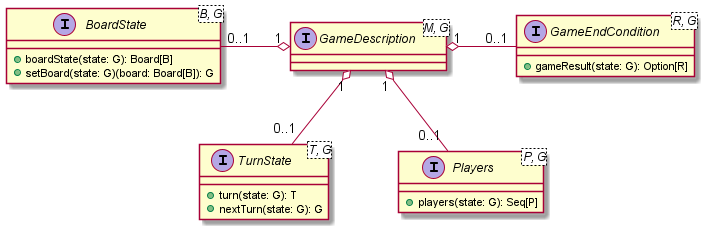
\includegraphics[width=\linewidth]{images/uml/extensions.png}
    \caption{Diagramma delle classi per le estensioni dello stato}
    \label{fig:extensions}
\end{figure}

% ---------------------------------------------------

\subsection{RuleSet e Dsl}\label{sec:dsl_design}

Si analizza ora il design di dettaglio relativo al \texttt{RuleSet} e al suo \textbf{DSL}.

Il \texttt{RuleSet} idendifica l'insieme delle regole che definiscono se, in un determinato stato, una \textit{move} è valida e in quale modo questa modifichi lo stato del gioco al momento della sua esecuzione (Requisiti \ref{req:dsl}).
%
La modalità con cui viene abilitato l'utilizzo del DSL, all'interno della definizione del proprio \texttt{RuleSet}, consiste nel dichiarare una classe (o un oggetto) che estenda dal trait \texttt{RuleSet} e aggiungere il trait \texttt{RuleSetBuilder} come mixin.
%
In questo modo, lo sviluppatore ha a disposizione una sintassi e un insieme di parole chiave definite dalla libreria.
%
La modalità scelta introduce, per il team, il problema di come organizzare le dichiarazioni delle parole chiave per fare in modo che la soluzione sia modulare e scalabile.
%
Il DSL, per questo motivo, è stato suddiviso in diverse componenti per mantenere un alto livello di modularità.
%
In seguito ciascuna componente è stata unificata, tramite l'utilizzo dell'ereditarietà multipla tramite mixin, in un unico trait (\texttt{RuleSetBuilder}) per consentire all'utente di abilitare l'intera sintassi con una sola dichiarazione.

Le componenti individuate sono descritte nei paragrafi seguenti.

\paragraph{MovesGeneration e MovesExecution}
Rappresentano il punto di collegamento tra il DSL e il \texttt{RuleSet}, poichè accumulano le varie regole scritte all'interno del sorgente in un unico punto e lo rendono disponibile per essere utilizzato come implementazione dell'interfaccia del \texttt{RuleSet}.

\subparagraph{Generators}
Un \texttt{Generator} rappresenta l'astrazione di base utilizzata per la generazione delle mosse ed è costituito da una funzione che, partendo da uno stato di gioco, genera un certo insieme di mosse valide (Requisito \ref{req:generator}).
%
Tramite la componente \texttt{Generators} viene fornita all'utente la sintassi per la creazione dei generatori più comuni.

\subparagraph{Actions}
Come la \texttt{MovesGeneration} è fondata sul concetto di \texttt{Generator} come astrazione base, così la componente \texttt{MovesExecution} è fondata sul concetto di \texttt{Action}.
%
Una \texttt{Action} è rappresentata da una funzione che, a partire da uno stato, restituisce un nuovo stato.
%
Le \texttt{Action} sono le azioni che saranno poi utilizzate per modificare lo stato come da requisito \ref{req:action}

Anche in questo caso, la componente \texttt{Actions} fornisce la sintassi per poter utilizzare le azioni più frequentemente impiegate nei giochi da tavolo.

\paragraph{Chainables e Modifiers}
Una volta forniti i mattoncini di base per la generazione e l'esecuzione delle mosse (rispettivamente \texttt{Generator} e \texttt{Action}), vengono forniti all'utente della libreria dei costrutti che consentono di combinare in diversi modi queste astrazioni.
%
Lo scopo è quello di permettere la creazione di azioni composite o di generatori più complessi, evitando di dover reinventare costantemente la ruota e riutilizzando il più possibile i meccanismi già implementati.

La soluzione fornita dalla libreria prevede la possibilità di \textbf{concatenare} tra di loro i meccanismi di base producendo nuove azioni o generatori, a loro volta combinabili.
%
Questa funzionalità è abilitata dalla type class \texttt{Chainable} (Figura \ref{fig:chainables}), che rappresenta una trasformazione \textbf{concatenabile} a un altra trasformazione dello stesso tipo.
%
\begin{figure}
    \centering
    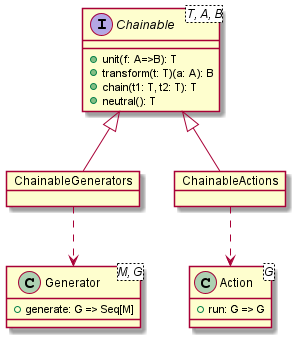
\includegraphics[width=0.5\linewidth]{images/uml/chainables.png}
    \caption{Diagramma delle classi contentente la struttura dei Chainable}
    \label{fig:chainables}
\end{figure}

Un tipo \texttt{Chainable} deve definire il modo in cui viene prodotto il risultato della concatenazione e deve inoltre definire il proprio \textbf{elemento neutro} (ovvero quello la cui concatenazione con qualsiasi altro elemento produce l'elemento stesso).
%
In questo possono essere considerati come dei \textbf{Monoidi}.
%
In più un \texttt{Chainable} è anche una trasformazione da un tipo \texttt{A} a un tipo \texttt{B}, entrambi definiti dall'istanza stessa di \texttt{Chainable}.
%
Il trait \texttt{Chainable} richiede quindi di definire un operatore \texttt{unit} che produce una trasformazione \texttt{T} a partire da una semplice funzione e un operatore \texttt{transform} che applica la trasformazione a un elemento.

Questa definizione consente di sfruttare il concetto di \texttt{Chainable} per permettere a generatori ed azioni di essere utilizzati all'interno dei \textbf{costrutti iterativi e condizionali} (\texttt{Modifiers}) messi a disposizione dal DSL della libreria.
%
I dettagli implementativi di come ciò avviene saranno descritti nella Sezione \ref{sec:dsl_syntax}.

\paragraph{Features}
Essendo il \texttt{RuleSet} definito a livello intensionale, è necessario avere un meccanismo per rappresentare le proprietà dello stato anche non avendo a disposizione una particolare istanza dello stesso.
%
Questa problematica è risolta dal concetto di \texttt{Feature}, ovvero una funzione che estrae dallo stato una sua proprietà.

La componente \texttt{Features} dichiara un insieme di \texttt{Feature} comunemente utilizzate.

% ---------------------------------------------------

\subsection{Interazione}

Le funzionalità abilitanti l'interazione con i giocatori sono state incapsulate totalmente nel modulo \texttt{interaction}, che comprende \texttt{view} e \texttt{controller}, con un interfacciamento verso il \texttt{model}.

Un gioco completo sviluppato con la libreria prevede due viste principali:
\begin{itemize}
    \item \textit{Menu}: il punto di ingresso dell'applicazione dove poter selezionare opzioni come giocare una nuova partita oppure uscire dal programma;
    \item \textit{Game}: una partita in corso.
\end{itemize}
%
Ciascuna di queste è composta da una specifica coppia di \texttt{SubView} e \texttt{SubController}.

\subsubsection{View}

La \texttt{View} principale è in grado di creare e inizializzare le \texttt{SubView} esponendo un metodo per ritornare ognuna di esse, semplificando la navigazione fra le \texttt{SubView}.

\paragraph{Menu view} 
È il componente per gestire tutto ciò che è precedente o successivo al \textit{Game} (es. avvio di un \textit{Game}, chiusura dell'applicazione).
%
Il \texttt{MenuView} permette tramite un'apposita UI di scegliere come procedere tra le varie opzioni.

\paragraph{Game view}

È la \texttt{SubView} responsabile della rappresentazione del gioco nel suo stato attuale e di gestire l'interazione con l'utente che inserisce dei comandi.

\subparagraph{Renderer}
Per effettuare il display dello stato del gioco, la \texttt{GameView} utilizza un certo insieme di \texttt{Renderer}, che sono responsabili della visualizzazione di uno specifico sottoinsieme delle informazioni da mostrare (Requisito \ref{req:renderers_parameters}).
%
Questa scelta è stata effettuata in quanto giochi diversi hanno proprietà diverse che devono essere mostrate all'utente, ed è necessario separare le diverse visualizzazioni al fine di renderle riutilizzabili e seguire il principio di singola responsabilità.
%
In particolare, quando le proprietà da visualizzare corrispondono alle \texttt{extension} è possibile utilizzare un \texttt{Renderer} comune a tutti i giochi con quella specifica estensione.
%
Richiamando l'aggiornamento di tutti i \texttt{Renderer} la \texttt{GameView} è in grado di mostare tutte le caratteristiche dello stato attuale del \textit{Game}.

\subparagraph{Event}
Ogni volta che un utente interagisce con la \texttt{GameView} inserendo dei comandi, quest'ultima genera degli \texttt{Event} che vengono ascoltati dal \texttt{GameController}.
%
Questo è a conoscenza del modo in cui convertire questi eventi in mosse da eseguire sullo stato o in altre azioni particolari.

% ---------------------------------------------------

\subsubsection{Controller}
I controller presentano una dipendenza dalle view in quanto devono chiamare i metodi della specifica \texttt{SubView} per fornire il feedback appropriato rispetto all'interazione intrapresa dal giocatore.
%
L'\texttt{ApplicationController} è responsabile di gestire la \texttt{View} principale, scegliendo quale \texttt{SubView} mostrare e aggiungendovi i \textbf{listener} relativi.

\paragraph{Menu controller}
Presenta le funzionalità per gestire l'avvio di una partita e la terminazione dell'applicazione.
%
Questo controller è una prima interfaccia con il \textbf{model}, che nel caso di avvio di una partita utilizza la \texttt{GameDescription} per la generazione di un nuovo \texttt{Game}.
%
Successivamente prepara la GameView con i parametri relativi, aggiunge un nuovo \texttt{GameController} come listener e passa alla nuova vista.

\paragraph{Game controller}
%
Come descritto in precedenza, il \texttt{GameController} gestisce gli \texttt{Event} che gli vengono notificati, presentando un comportamento diverso in base alla situazione (Requisito \ref{req:events}):
%
\begin{itemize}
    \item Se l'evento è \texttt{Quit} allora termina la \texttt{GameView}.
    \item Se l'evento è \texttt{Undo} allora annulla l'ultima mossa eseguita.
    \item In tutti gli altri casi, gli eventi vengono accodati fino a che non vengono riconosciuti come mossa.
\end{itemize}
%
Quando viene riconosciuta una mossa, la coda degli eventi viene svuotata e la mossa viene eseguita (tramite \texttt{executeMove}) sull'istanza corrente del \texttt{Game}, producendo due possibilità:
\begin{itemize}
    \item se la mossa è valida per lo stato attuale del gioco, viene eseguita e la chiamata restituisce il nuovo stato prodotto;
    \item se la mossa non è valida o se viene lanciata un'eccezione durante l'esecuzione, viene restituita una failure che descrive cosa non ha funzionato.
\end{itemize}
%
In entrambi i casi il risultato della chiamata viene comunicato alla \texttt{GameView} chiamando un metodo tra \texttt{moveAccepted} o \texttt{moveRejected}.
%
La Figura \ref{fig:gui_sequence} mostra più schematicamente come avviene questa interazione.
\begin{figure}
  \centering
  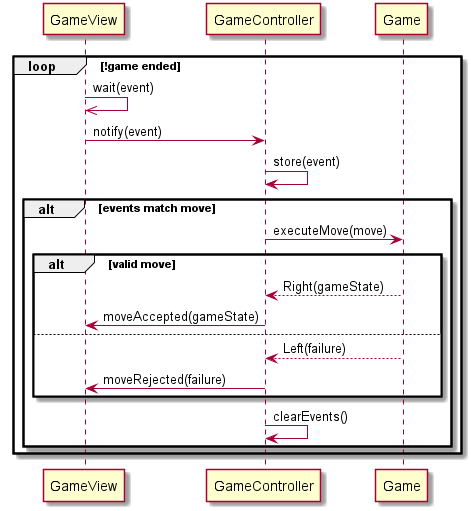
\includegraphics[width=\linewidth]{images/uml/gui_sequence.png}
  \caption{Diagramma di sequenza rappresentante le interazioni in un game tra model, view e controller}
  \label{fig:gui_sequence}
\end{figure}


